\newpage
\subsubsection{Caso d'uso UC4.1: Login tramite API Market}
\label{UC4_1}
\begin{figure}[!htbp]
	\centering
	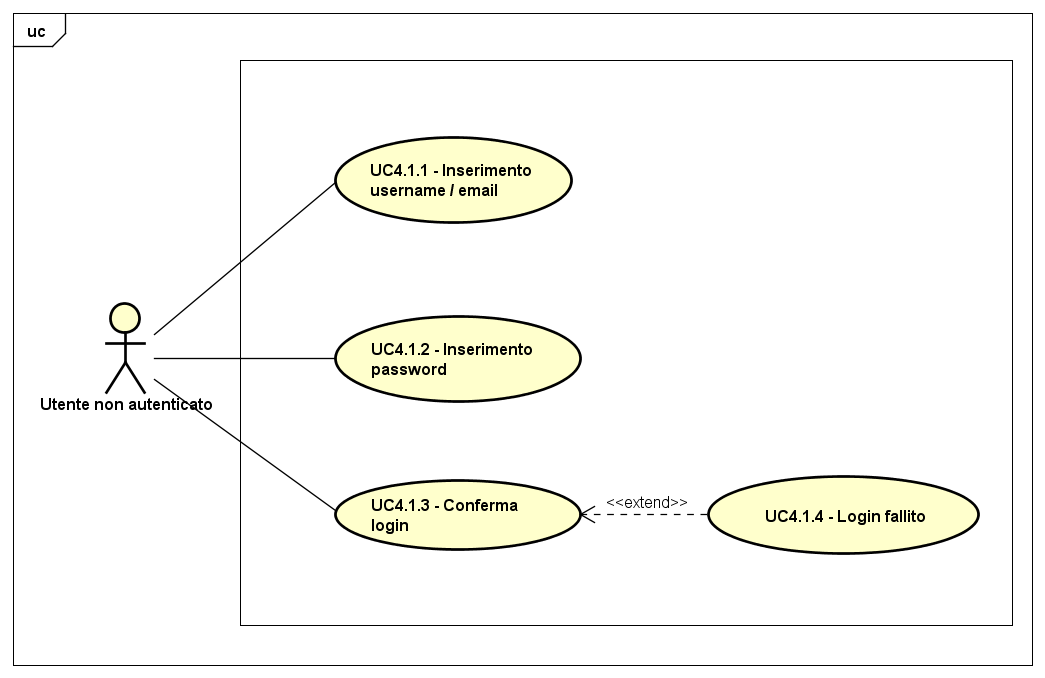
\includegraphics[scale=0.45]{UML/UC4_1.png}
	\caption{UC4.1: Login tramite API Market}
\end{figure}

\begin{tabular}{ l | p{11cm}}
	\hline
	\rowcolor{Gray}
	 \multicolumn{2}{c}{UC4.1 - Login tramite API Market} \\
	 \hline
	\textbf{Attori} & Utente non autenticato \\
	\textbf{Descrizione} & L'attore effettua il login all'applicazione web, così da evolversi in un utente autenticato\\
	\textbf{Pre-Condizioni} & L'attore ha scelto di eseguire il login all'applicazione web e non è autenticato \\
	\textbf{Post-Condizioni} & L'attore ha effettuato il login all'applicazione web, evolvendosi in un utente autenticato \\
	\textbf{Scenario Principale} & 
	\begin{enumerate*}[label=(\arabic*.),itemjoin={\newline}]
		\item L'attore può inserire l'email o username (UC4.1.1)
		\item L'attore non autenticato può inserire la password (UC4.1.2)
		\item L'attore può confermare i dati inseriti per procedere al login (UC4.1.3)
	\end{enumerate*}\\
\end{tabular}


\paragraph{Caso d'uso UC4.1.1:  Inserimento username o email}
\label{UC4_1_1}

\begin{minipage}{\linewidth}
\begin{longtable}{ l | p{11cm}}
	\hline
	\rowcolor{Gray}
	\multicolumn{2}{c}{Caso d'uso UC4.1.1:  Inserimento username o email} \\
	\hline
	\textbf{Attori} & Utente non autenticato \\
	\textbf{Descrizione} & L'attore inserisce la propria username o email  \\
	\textbf{Pre-Condizioni} & L'applicazione visualizza i form per l'inserimento del campo per lo username \\
	\textbf{Post-Condizioni} & L'attore ha inserito il proprio username o email \\
	\textbf{Scenario Principale} & \begin{enumerate*}[label=(\arabic*.),itemjoin={\newline}]
		\item L'utente non autenticato può inserire il proprio username o la propria email
	\end{enumerate*}\\
\end{longtable}
\end{minipage}


\paragraph{Caso d'uso UC4.1.2:  Inserimento password}
\label{UC4_1_2}

\begin{minipage}{\linewidth}
\begin{longtable}{ l | p{11cm}}
	\hline
	\rowcolor{Gray}
	\multicolumn{2}{c}{Caso d'uso UC4.1.2:  Inserimento password} \\
	\hline
	\textbf{Attori} & Utente non autenticato \\
	\textbf{Descrizione} & L'attore inserisce la propria password  \\
	\textbf{Pre-Condizioni} & L'applicazione visualizza i form per l'inserimento del campo per la password \\
	\textbf{Post-Condizioni} & L'attore ha inserito la propria password \\
	\textbf{Scenario Principale} & \begin{enumerate*}[label=(\arabic*.),itemjoin={\newline}]
		\item L'utente non autenticato può inserire la propria password
	\end{enumerate*}\\
\end{longtable}
\end{minipage}


\paragraph{Caso d'uso UC4.1.3:  Inserimento username o email}
\label{UC4_1_3}

\begin{minipage}{\linewidth}
\begin{longtable}{ l | p{11cm}}
	\hline
	\rowcolor{Gray}
	\multicolumn{2}{c}{Caso d'uso UC4.1.3:  Inserimento username o email} \\
	\hline
	\textbf{Attori} & Utente non autenticato \\
	\textbf{Descrizione} & L'attore conferma i dati inseriti per il login  \\
	\textbf{Pre-Condizioni} & L'applicazione visualizza il pulsante per confermare i dati di accesso \\
	\textbf{Post-Condizioni} & L'attore ha confermato i dati inseriti \\
	\textbf{Scenario Principale} & \begin{enumerate*}[label=(\arabic*.),itemjoin={\newline}]
	\item L'attore convalida i dati inseriti per procedere con il login, e verrà reindirizzato alla schermata principale post-autenticazione (UC2) oppure, in caso di login fallito, viene consentito all'utente di ritentare dall'apposita schermata (UC4.1)
\end{enumerate*}\\
\end{longtable}
\end{minipage}